% ---------------------------------------------------------------- cover
\thispagestyle{empty}
\AddToShipoutPictureBG*{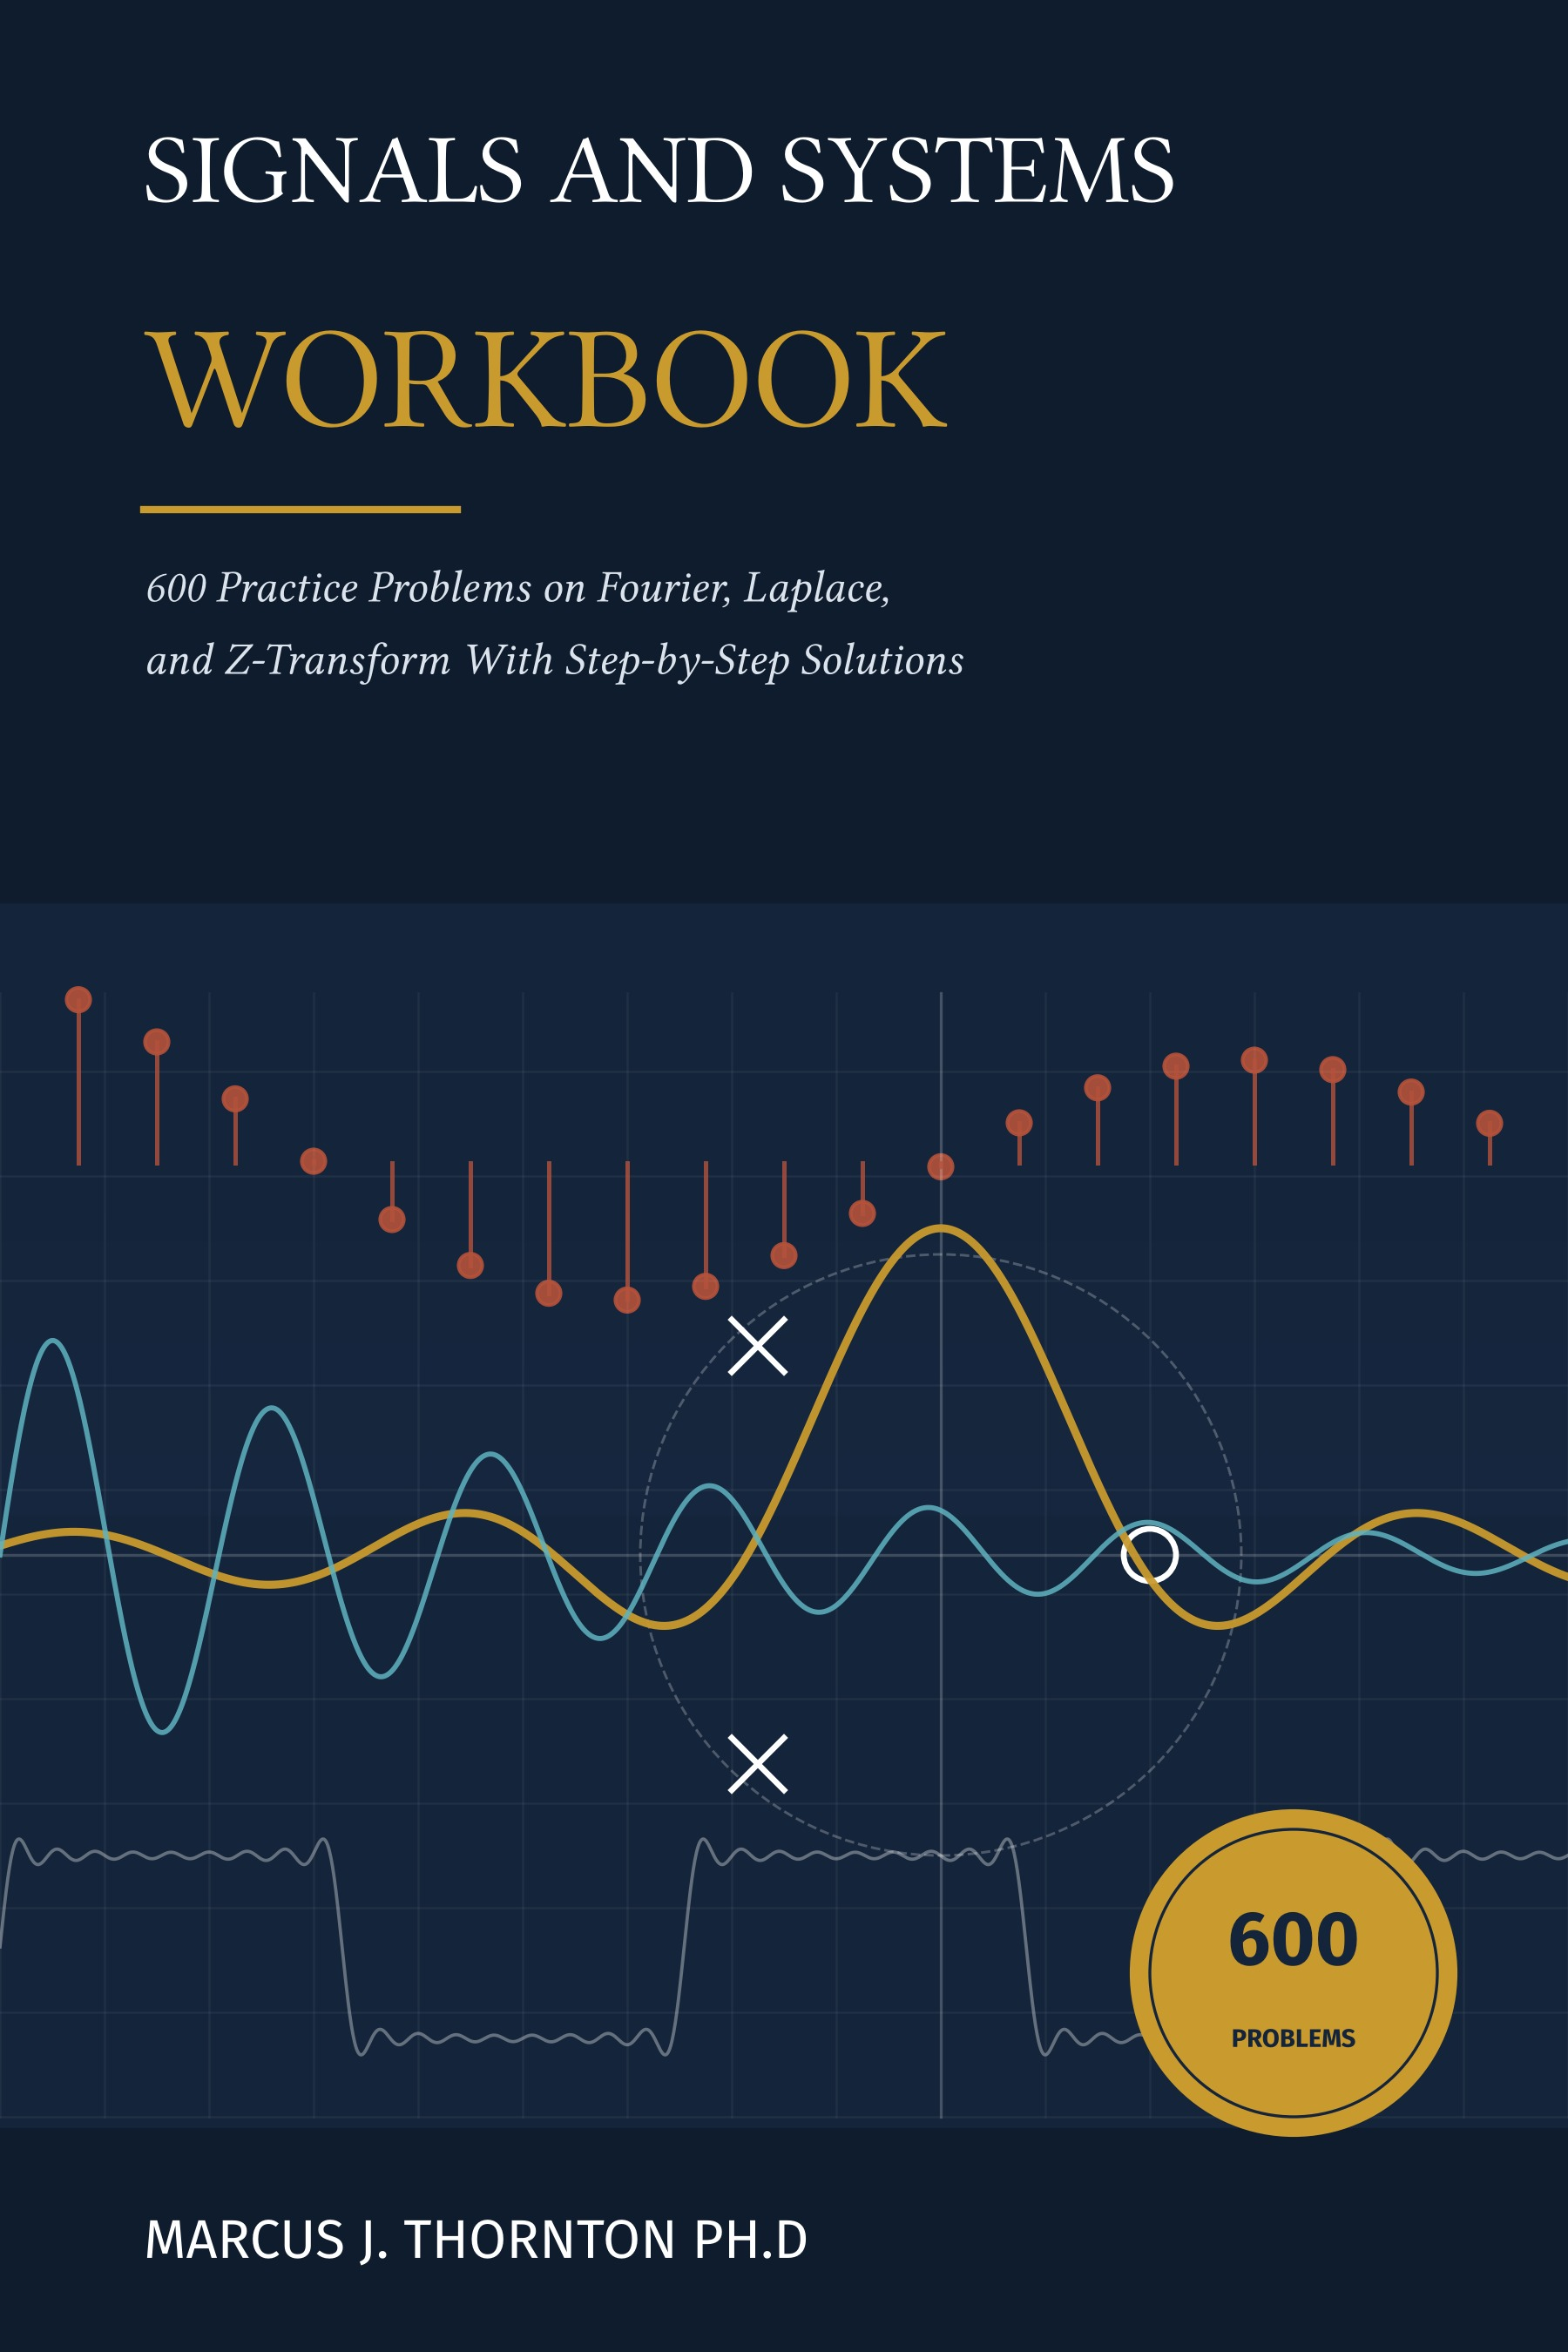
\includegraphics[width=\paperwidth,height=\paperheight]{output/cover.jpg}}
\mbox{}
\clearpage
\thispagestyle{empty}\mbox{}\clearpage
% ---------------------------------------------------------------- half title
\thispagestyle{empty}
\vspace*{1.6in}
\begin{center}
{\displayfont\fontsize{22}{27}\selectfont\color{navy}Signals and Systems Workbook\par}
\vspace{10pt}{\color{gold}\rule{0.9in}{1pt}}
\end{center}
\clearpage
\thispagestyle{empty}
\vspace*{1.2in}
\begin{center}
{\sffamily\scriptsize\addfontfeature{LetterSpace=18}\color{greyc}ALSO FOR THE WORKING ENGINEER\par}
\vspace{14pt}
\begin{minipage}{0.78\linewidth}\centering\small\itshape
This workbook is written for the student who has sat through the lectures, nodded along,
and then found that the problem sheet is a different animal altogether.
It is equally for the practising engineer who wants the mathematics back at their fingertips.
\end{minipage}
\end{center}
\clearpage
% ---------------------------------------------------------------- title page
\thispagestyle{empty}
\begin{tikzpicture}[remember picture,overlay]
  \fill[navy] (current page.north west) rectangle ([yshift=-2.15in]current page.north east);
  \begin{scope}[shift={([yshift=-2.15in]current page.north west)}]
    \draw[gold,line width=0.8pt,domain=0:15.24,samples=200,smooth] plot (\x,{0.55*exp(-0.15*\x)*sin(160*\x)+0.75});
  \end{scope}
\end{tikzpicture}
\vspace*{1.95in}
\begin{flushleft}
{\displayfont\fontsize{30}{35}\selectfont\color{navy}Signals and Systems\\ Workbook\par}
\vspace{14pt}{\color{gold}\rule{1.1in}{1.2pt}}\par\vspace{14pt}
{\large\itshape\color{ink}600 Practice Problems on Fourier, Laplace,\\ and Z-Transform With Step-by-Step Solutions\par}
\vfill
{\sffamily\large\color{navy}Marcus J. Thornton\,\textsc{ph.d}\par}
\vspace{0.3in}
\end{flushleft}
\clearpage
% ---------------------------------------------------------------- copyright
\thispagestyle{empty}
\vspace*{\fill}
{\footnotesize\setlength{\parindent}{0pt}\setlength{\parskip}{6pt}
\textbf{Signals and Systems Workbook}\\
\textit{600 Practice Problems on Fourier, Laplace, and Z-Transform With Step-by-Step Solutions}

Copyright \textcopyright\ 2026 Marcus J. Thornton. All rights reserved.

No part of this publication may be reproduced, stored in a retrieval system or transmitted in any form or by any
means, electronic, mechanical, photocopying, recording or otherwise, without the prior written permission of the
author, except for brief quotations embodied in critical articles and reviews.

Every effort has been made to ensure that the solutions in this book are accurate. The methods, worked answers and
examples are provided for educational purposes. The author accepts no liability for any loss arising from the use
of this material in the design of real systems, which should always be verified independently.

Written in British English.

First edition, 2026.

Typeset in Libertinus Serif and Fira Sans. Illustrations by the author.
\par}
\clearpage
% ---------------------------------------------------------------- dedication
\thispagestyle{empty}
\vspace*{2in}
\begin{center}\itshape\color{navy}
For every student who has stared at a partial fraction\\ at two in the morning and refused to give up.
\end{center}
\clearpage
% ---------------------------------------------------------------- contents
{\hypersetup{linkcolor=ink}
\renewcommand{\contentsname}{Contents}
\tableofcontents}
